\documentclass[12pt,letterpaper]{article}
\usepackage[utf8]{inputenc}
\usepackage{amsmath,amssymb,amsthm}
\usepackage{graphicx}
\usepackage{natbib}
\usepackage{pgfplots}  % For generating graphs within LaTeX
\usepackage{hyperref}
\usepackage{setspace}
\usepackage{booktabs}
\usepackage{float}
\usepackage{geometry}

\title{The Market for Elite Status}
\author{Joao Faria and Michael Ryall}
\date{\today}

\begin{document}
	
	\maketitle

	
%	\begin{abstract}
%		Blah blah blah...
%	\end{abstract}
	
	\onehalfspacing
	
\section{Introduction}
	\section{Introduction}
	
	Why do elite institutions persist when they appear to underperform their non-elite counterparts? From investment banks that hire exclusively from Ivy League schools to consulting firms that charge premium fees despite questionable value-added, many markets exhibit a puzzling pattern: organizations that signal elite status command substantial premiums while potentially delivering inferior outcomes. Standard economic theory suggests that competitive forces should eliminate such inefficiencies, yet these patterns not only persist but often dominate entire industries.
	
	This paper develops a theoretical framework to explain how markets for elite status can sustain inefficient equilibria in competitive environments. We argue that when agents derive utility from membership in high-status groups, the resulting sorting patterns can create self-reinforcing cycles that insulate inefficient elite organizations from competitive pressure. The key insight is that elite status functions as both a consumption good (providing direct utility to members) and a signaling device (affecting how others perceive and interact with members), creating complementarities that allow inefficient equilibria to persist indefinitely.
	
	Our analysis proceeds through two complementary approaches. First, we develop a static general equilibrium model using the club goods framework to characterize the conditions under which inefficient elite equilibria exist. We model an economy with four types of organizations: elite universities that provide status but minimal skill development, serious universities that build genuine human capital, elite firms managed by graduates of elite universities, and competent firms managed by graduates of serious universities. Despite elite firms being less productive in terms of resource utilization, they can survive and prosper because agents are willing to pay premium prices to work with other elite members.
	
	Second, we extend this framework to a dynamic overlapping generations setting where agents make intertemporal education investment decisions. This dynamic perspective reveals how elite status markets can exhibit path dependence and multiple equilibria, with initial conditions determining whether an economy converges to an efficient or inefficient steady state. The dynamic model also illuminates the welfare costs of elite competition and suggests potential policy interventions.
	
	Our main theoretical results establish three key findings. First, inefficient elite equilibria can exist and be stable when agents sufficiently value elite status relative to consumption. Second, these equilibria are characterized by systematic resource misallocation: elite institutions consume excessive resources to signal their status, while elite managers command wage premiums that exceed their marginal productivity. Third, the welfare costs of elite competition can be substantial, as resources are diverted from productive uses toward status signaling activities.
	
	The model generates several empirically testable predictions. Elite institutions should charge higher fees but deliver lower value-added per dollar spent. Elite managers should receive compensation premiums that correlate with the exclusivity of their educational background rather than measured productivity. Industries with stronger elite preferences should exhibit greater price dispersion and lower overall productivity. Markets should display persistent segmentation along elite/non-elite lines, with limited mobility between segments.
	
	These findings have important implications for policy. Traditional antitrust approaches may be ineffective against elite cartels because the inefficiency stems from demand-side status preferences rather than supply-side market power. Instead, policies that reduce status signaling incentives or increase transparency about institutional performance may be more effective. Educational policies that strengthen the signaling value of non-elite institutions could also help redirect talent toward more productive uses.
	
	Our framework contributes to several strands of economic literature. Most directly, it extends models of club goods and social groups to analyze market equilibrium with endogenous group formation. It also connects to the extensive literature on signaling and screening in labor markets, though our focus on group membership rather than individual characteristics represents a novel perspective. The dynamic analysis contributes to the literature on social mobility and intergenerational transmission of advantage.
	
	The remainder of the paper is organized as follows. Section 2 presents the static general equilibrium model and characterizes the conditions for existence of elite equilibria. Section 3 develops a numerical example to illustrate the key mechanisms and provide comparative statics results. Section 4 extends the analysis to a dynamic setting and examines stability and welfare properties. Section 5 discusses empirical implications and policy relevance. Section 6 concludes.

	
	
	
\section{Notation at a Glance}\label{sec:notation}

\begin{table}[H]\centering
	\small
	\begin{tabular}{@{}p{2.8cm}p{10cm}@{}}
		\toprule
		\multicolumn{2}{c}{\textbf{Static (General-Equilibrium) Objects}}\\
		\midrule
		$y_1$ & Input / “money’’ good (resource units).\\
		$y_2$ & Output / consumption good.\\
		$k$ & Per-capita endowment of $y_1$.\\
		$r$ & Resource cost per student in a \emph{serious} university.\\
		$\tau r$ & Resource cost per student in an \emph{elite} university ($\tau\!\ge1$).\\
		$c$ & Input requirement of a competent firm.\\
		$\phi$ & Output of a competent firm.\\
		$\beta$ & Input inefficiency multiplier for elite firms ($\beta\!\ge1$).\\
		$\alpha$ & Output multiplier for elite firms.\\
		$q_i$ & Prices of memberships (tuition fees, wages).\\
		$\sigma_j$ & Population shares choosing each vocation ($j=0,1,2$).\\
		\midrule
		\multicolumn{2}{c}{\textbf{Dynamic (Overlapping-Generations) Extensions}}\\
		\midrule
		$k_t$ & Household holdings of $y_1$ (“wealth’’) at date $t$.\\
		$c_{1t}$, $c_{2,t+1}$ & Consumption of $y_2$ in periods $t$ and $t\!+\!1$.\\
		$s_t$ & Tuition expenditure (units of $y_1$) paid at $t$.\\
		$\theta$ & Ability / status parameter ($\theta\!\in[\underline{\theta},\overline{\theta}]$).\\
		$\hat{\beta}$ & \emph{Intertemporal} discount factor $1/(1+\rho)\in(0,1)$  
		\newline (distinguished from the static $\beta$ above).\\
		$\mathcal{R}_{t+1}$ & Gross return on equity between $t$ and $t\!+\!1$.\\
		$\delta$ & Marginal-cost parameter in college production.\\
		$\varphi_t$ & College net income at date $t$.\\
		$\sigma$ & Weight of stock-holder “style’’ preference in firm objective.\\
		$K_t,\;k_t$ & Industry-wide and firm-specific capital stocks.\\
		\bottomrule
	\end{tabular}
	\caption{Key symbols used throughout the paper.  A hat marks dynamic symbols that would otherwise clash with static ones.}
\end{table}
	
	\section{General model}
	I will approach this in two steps. 
	First, I will map Ellickson et al. (2007) to our  general case (i.e., as a special case of the Ellickson et al. general model but as the general case of concern to us).
	Second, I will work through some numerical examples.
	
	\subsection{Groups and memberships}
	There are two divisible, publicly traded private goods, $y_1$ and $y_2$, which we can think of as money and a consumption good. Then, $y=(y_1,y_2)\in\mathbb{R}^2$.
	
	There are four group types: i) the group of the socially elite; ii) \textit{Elite degree mills}; iii) \textit{Serious universities}; and iv) \textit{firms}.
	Group types are defined by their membership characteristics and organizational characteristics.
	
	Let $\Omega$ and $\Gamma$ be finite sets of \textit{membership characteristics} and \textit{organizational characteristics}, respectively. 
	A \textit{group type} is a triple $(\pi,\gamma,y)$ consisting of a \textit{profile} $\pi:\Omega\rightarrow\{0,1,\ldots\}$, an \textit{organizational characteristic} $\gamma\in\Gamma$, and an \textit{input-output vector} $y\in\mathbb{R}^2$.
	There will be a finite set of possible group types $\mathcal{G}=\{(\pi,\gamma,y)\}$.
	
	For $\omega\in \Omega$, $\pi(\omega)$ represents the number of members with the membership characteristic $\omega$ that the group is required to have, so $|\pi|=\sum_{\omega\in\Omega}\pi(\omega)$ is the total number of members that the group is required to have.\footnote
		{
		``A membership characteristic is anything that matters to the individual who comprise a group or to the activity in which the group is engaged. In particular, a membership characteristic can encompass personal qualitites qualities (intelligence, appear- ance, personality, etc.), roles within the group (teacher, student, supervisor, skilled laborer, unskilled laborer, etc.) and skills (singing, dancing, language, etc.). Formally, all membership characteristics are acquired; membership characteristics that are innate (height for instance) are encompassed in our specification of consumption sets below. [In our earlier paper, we insisted that membership characteristics be innate and fixed.] Importantly, membership characteristics are observable and contractible. We emphasize that $\Omega$ is simply an abstract finite set. In particular, $\Omega$ is not a vector space and need not have any linear structure.''
	}
	
	In this case, it seems that what we need is fairly straightforward in terms of groups and requisite membership characteristics:
	\begin{enumerate}
		\item \textit{Elite degree mills} take in students, no membership characteristics required, and confer elite status (but have no effect on managerial skills). 
		\item \textit{Serious universities} also take in anyone. These confer actual managerial skill.
		\item The \textit{socially elite} requires having completed education in an Elite degree mill.
		\item \textit{Firms} will require managers and laborers. Managers are those who graduate from a university. Those from serious universities are more productive. 
	\end{enumerate}
	It would also be interesting to introduce high and low quality faculty and see where they migrate, but not for now.\footnote
	{ 
		``An organizational characteristic might be anything that matters to the potential member of a group apart from the characteristics of the members in the group and the input-output vector. In particular, an organizational characteristic can encompass the activity within the group (that is, the process used to produce output), the organizational hierarchy within the group, and the duties of each potential member of the group.''
	}
	Clearly, elites will want to be with other elites in firms -- this is a key part of the model. 
	We might even assume that laborers prefer \textit{not} to work in firms run by elites.
	But, these are characteristics of firm members.
	So, the only things that seem to fit the requirements for organizational characteristic are the university processes (degree mills or actual learning centers).
	These are organizational characteristics because they are not determined by member characteristics or the input-output vector.
	Colleges produce ``education'' (of one form or the other) and take tuition.
	[Not clear if education is also a publicly traded good.]
	Firms, of course, produce products and pay wages.
	
	A membership is a pair $m=(\omega,(\pi,\gamma,y))$ such that $(\pi,\gamma,y)\in\mathcal{G}$ and $\pi(\omega)\ge 1$. Let $\mathcal{M}$ be the finite set of group memberships. Agents choose a bundle of memberships, referred to as a \textit{list}, which is a function $l:\mathcal{M}\rightarrow\{0,1,\ldots\}$; $l(m)$ specifies the number of memberships of type $m=(\omega,(\pi,\gamma,y))$.
	The set of lists is denoted \textbf{Lists}.
	
	\subsection{Agents}
	The set of agents is a nonatomic finite measure space $(A,\mathcal{F},\lambda)$: $A$ is a set, $\mathcal{F}$ a $\sigma$-algebra of subsets of $A$, and $\lambda$ is a non-atomic measure on $\mathcal{F}$ with $\lambda(A)<\infty$.
	A complete description of $a\in A$ consists of a \textit{consumption set}, an \textit{endowment vector} of private goods, and a \textit{utility function}. 
	
	\subsubsection{Consumption sets}
	Agent $a$'s consumption set $X_a$ specifies the feasible pairs of bundles of private goods and lists of membership that the agent may choose.
	Assume the following:
	\begin{enumerate}
		\item $X_a\subset\mathbb{R}^2_+\times\textbf{Lists}$,
		\item If $(x_a,\mu_a)\in X_a$ and $x^\prime_a\ge x_a$ then $(x^\prime_a,\mu_a)\in X_a$,
		\item There exists $M>0$ such that for all $a\in A$ and all $(x_a,\mu_a)\in X_a$
		\[
		\sum_{m\in\mathcal{M}}\mu_a(m)\le M.
		\]
	\end{enumerate}
	The first condition says private good consumption must be nonnegative. 
	The second says increased consumption of private goods is always possible.
	The last says that the number of memberships each agent can choose is bounded.
	In particular, for each agent $a\in A$, the set
	\[
	\textbf{Lists}_a\equiv\{\mu_a\in\textbf{Lists}|\exists x_a\in \mathbb{R}^2_+ \text{ s.t. }(x_a,\mu_a)\in X_a\}
	\]
	is finite.\footnote
	{
		``A choice $(x_a,\mu_a)$ is in $X_a$ if it is possible for agent $a$ to consume the bundle of private goods $x_a$ and fulfill the requirements of the memberships specified by $\mu_a$.
		The consumption set $X_a$ encodes restrictions on the choices that $a$ can make with respect to both private goods and memberships.''
	}
	
	In our setting, elite education is required for being part of the elite group.
	In addition, any education is required to be in the managerial class.
	Let $f,f^\ast,s,s^\ast\in\mathcal{G}$ be a firm,  an elite firm, a serious school of higher education, and an elite degree mill, respectively.
	Then, $(\omega,f)$ requires that $\omega$ be ``holds a college degree of either kind.''
	
	Thus, we insist that if $(\mu_a,f)\in X_a$ and $\mu_a(\omega,f)>0$, then $\mu_a(\omega^\prime,s)>0$ or  $\mu_a(\omega^\prime,s^\ast)>0$.
	Similarly, if $(\mu_a,f^\ast)\in X_a$ and $\mu_a(\omega,f^\ast)>0$, then $\mu_a(\omega^\prime,s^\ast)>0$.
	(It is for this reason that we cannot assume $X_a=\mathbb{R}^2_+\times\textbf{Lists}$.)\footnote
	{
		``Much of the flexibility of our model arises from the fact that an agent can choose (memberships with) different characteristics in different groups. In particular, we allow an agent to fill different roles in different groups — to provide barber services in one group and receive them in another. The possibility of filling different roles in different groups is essential to the way we model the acquisition of skills, which will typically be acquired in one venue and applied in another. Of course, the acquisition of skills usually precedes their application; we incorporate the temporal element by viewing the date or time period as part of the description of a group, just as traditional general equilibrium theory frequently views the date or time period as part of the description of a commodity.''
	}
	This suggests that part of the descriptions of schools include a date $t$ and of firms a date $t+1$.
	
	\subsubsection{Endowments}
	Agent $a$'s \textit{endowment} is $(e_a,0)\in X_a$. 
	Agents are endowed with private goods but not with group memberships.

	\subsubsection{Utility functions}
	Agent $a$'s \textit{utility function} is $u_a:X_a\rightarrow \mathbb{R}$ is defined over private goods conumptions and lists of group membership.
	Assume, for each $\mu_a\in\textbf{ Lists}$,
	\[
	 u_a(\cdot,\mu_a):\{x_a|(x_a,\mu_a)\in X_a\}\rightarrow \mathbb{R}
	 \]
	 is continuous and strictly monotone; i.e., utility is strictly increasing in consumption of private goods.
	 No assumptions are made about the way in which utility depends on the choice of group memberships.
	 
	 \subsection{Economies}
	 An \textit{economy} $\mathcal{E}$ is a mapping $a\mapsto(X_a,e_a,u_a)$ for which:
	 \begin{itemize}
	 	\item The consumption set correspondence $a\mapsto X_a$ is a measurable correspondence.
	 	\item The endowment mapping $a\mapsto e_a$ is an integrable function.
	 	\item The utlity mapping $(a,x,l)\mapsto u_a(x,l)$ is a jointly measurable function of its arguments.
	 \end{itemize}
	 We may  that agents begin only with an endowment of money (e.g., $Y$ in our dynamic model).
	 
	 \subsection{States}
	 A \textit{state} of an economy is a measurable mapping
	 \[
	 (x,\mu):A\rightarrow \mathbb{R}^2\times\mathbb{R}^\mathcal{M}.
	 \]
	A state specifies choices of private goods and group memberships.
	Feasibility of a state of the economy is defined as feasibility of the consumption and productions plans and consistent matching of agents.
	In our case, we will require that there be some fixed fraction of managers to workers for the set of firms (i.e.g, because the set of agents is a continuum).
	Of course, we can have different types of firm and these can have production technologies that require a different ratio of managers to workers.
	
	To formalize this idea, define the \textit{membership vector} $\bar{\mu}\in \mathbb{R}^\mathcal{M}$.
	An aggregate membership vector $\bar{\mu}$ is consistent if for every group type $(\pi,\gamma,y)\in\mathcal{G}$, there is a real number $\alpha(\pi,\gamma,y)$,
	\[
	\bar{\mu}(\omega,(\pi,\gamma,y))=\alpha(\pi,\gamma,y)\pi(\omega)
	\]
	for each $\omega\in\Omega$. Given a measurable set $B\subset A$ and a measurable choice function $\mu:B\rightarrow\textbf{Lists}$, we say that $\mu$ is \textit{consistent for} $B$ if the aggregate membership vector $\int_B\mu_ad\lambda(a)$ is consistent.
	
	Then, $(x,\mu)$ is \textit{feasible for} the measurable subset $B\subset A$ if
	\begin{enumerate}
		\item \textbf{Individual feasibility}:  $(x_a,\mu_a)\in X_a\text{ for each } a\in B$
		 \item \textbf{Material balance}: 
		 \[
		 \int_B x_a d\lambda(a)\le \int_B e_a d\lambda(a) + 
		 \left[
		 \sum_{(\omega,(\pi,\gamma,y))} \mu_a(\omega,(\pi,\gamma,y))\frac{y}{|\pi|}
		 \right]d\lambda(a).
		 \]
		 \item \textbf{Consistency}: $\int_B\mu_a d\lambda(a)$ is consistent for $B$.
	\end{enumerate}
	Item 1 says $(x,\mu)$ is feasible for $B$ if individuals in $B$ choose profiles in their consumption sets, private consumption does not exceed the sum of endowments, and net production and agents are matched consistently.
	The state $(x,\mu)$ is \textit{feasible} if this condition applies to $A$.
	If $(x,\mu)$ is  a state of  the economy, $m=(\omega,g)$ is a membership and $\mu_a(m)>0$, $a$ is said to \textit{choose} the membership $m$.
	
	If $(x\mu)$ is consistent for $B$ and $\int_B \mu_a d\lambda(a)=\alpha(\pi,\gamma,y)\pi(\omega)$ for each $\omega\in\Omega$, then material balance is equivalent to the assertion that 
	\[
	\int_B x_a d\lambda(a)\le \int_B e_a d\lambda(a) + 
	\sum_{(\pi,\gamma,y)\in\mathcal{G}} \alpha(\pi,\gamma,y)y.
	\]
	Members of a group only consider the membership characteristics of other members and their identities
	Therefore, it is not necessary to identify the agents belonging to each group by individual.
	
	\subsection{Group equilibrium}
	Both private goods and group memberships are priced, so prices $(p,q)\in\mathbb{R}^2\times\mathbb{R}^\mathcal{M}$.
	In other words, $p$ is the vector of prices for private goods and $q$ is the vector of prices for group memberships.\footnote 
	{
		``Because utility functions are assumed monotone in private goods, private goods prices will be positive in equilibrium, but prices of group memberships may be positive, negative or zero. Because a membership specifies both a group type and a membership characteristic, membership prices depend both on the group type and the membership characteristic.''
	}
	
	A group equilibrium consists of prices $(p,q)\in\mathbb{R}^2\times\mathbb{R}^\mathcal{M}$, with $p\ne 0$ and a feasible state $(x,\mu)$ such that 
	\begin{enumerate}
		\item \textbf{Budget balance for group types}: For each $(\pi,\gamma,y)\in\mathcal{G}$:
		\[
		\sum_{\omega\in\Omega}\pi(\omega)q(\omega,(\pi,\gamma,y))+p\cdot y=0.
		\]
		\item \textbf{Budget feasiblity for agents}: For almost all $a\in A$,
		\[
		(p,q)\cdot(x_a,\mu_a)\le p\cdot e_a.
		\]
		\item \textbf{Optimization by agents}: For almost all $a\in A$,
		\[
		(x^\prime_a,\mu^\prime_a)\text{ and } u_a(x_a,\mu_a)\Rightarrow (p,q)\cdot	(x^\prime_a,\mu^\prime_a)>p\cdot e_a.
		\]		
	\end{enumerate}
	In other words, in equilibrium the sum of membership prices in a given group type just balances the value of the input-output vector and individuals optimize subject to their budget constraints.
	
	\section{Details for our case}
	
	\subsection{Agents}
	Assume a continuum of agents $A$. 
	All agents are ex-ante identical. 
	Each has endowment $e=(k,0)\in\mathbb{R}^2_+$, where we can think of $k$ as the (per capita) wealth of the economy.
	The first component is the quantity of input (a resource good) and the second is the quantity of output (a consumption good).
	
	\subsection{Groups}
	The indexed set of membership characteristics is  $\Omega=\{\omega_1,\ldots,\omega_4\}$ where  $\omega_1=S$ represents a student at a university, $\omega_2=M$ a manager, $\omega_3=EM$ an elite manager, and $\omega_4=L$ a laborer.
	
	There are four group types. 
	Serious schools are type $g_1=((S),s,y_s)$, in which the only member role is $\pi_s=(S)$, a student, and $y_s=(-r,0)$ because the university requires basic inputs of $r\ge 0$ to educate an individual student.\footnote
	{
		Note that writing $\pi_s=(S)$ is another abuse of notation since $\pi$ is a profile; i.e., $\pi_s=(1,0,0,0)$ is the technically correct, but more cumbersome, representation.
	}
	Similarly, $g_2=((S),s^\ast,y_{s^\ast})$ with  $y_{s^\ast}=(- \tau  r,0)$, where $\tau\ge 1$ is a parameter that accounts for the possibility that elite universities consume more resources than serious universities (on such things as beautiful facilities in geographically expensive areas, research faculty who do relatively little teaching, etc).
	
	Firms are also of two types, those run by well-trained managers and those run by elite managers.
	Let $g_3=((M,2L),f,y_f)$, which indicates that one manager and two laborers are required to staff a firm.
	Then $y_f=(-y_{f1},y_{f2})$ is the competent firm's production function in which $y_{f1}$ units of the input good are required to produce$y_{f2}$ units of the output good.
	Specifically, assume $y_f=(-c,\phi)$ where $\phi$ is the basic level of output common to both firm types.
	
	Similarly, there is a type of firm run by elite managers,   $g_4=((EM,2L),f,y_{f^\ast})$, in which one manager and two laborers are required and $y_{f^\ast}=(- \beta c,\alpha\phi)$ where $\beta\ge 1$ is a multiplier that accounts for input productivity differentials between the firm types (e.g, $\beta>1$ would reflect the fact that because elite universities do not actually teach anything, elite managers run their businesses less efficiently, such as by engaging in  signaling elite status by wasting firm resources in public displays of elite solidarity).
	Similarly,   $\alpha\ge 0$ is a multiplier that allows us to account for an output productivity differential between firms
	
	The set of possible group memberships, $\mathcal{M}$, contains the following elements:
	\begin{align*}
		&m_1=(S,g_1),m_2=(S,g_2),\\
		&m_{3.1}=(M,g_3),m_{3.2}=(L,g_3),\\
		&m_{4.1}=(EM,g_4),m_{4.2}=(L,g_4).
		.
	\end{align*}
	We assume that no agent can attend more than one university or work for more than one firm as either a manager or a laborer.
	Managers are those that attended a serious university and elite managers must have attended an elite university. 
	Thus, for all individuals,
	\begin{align*}
		\textbf{Lists}=\Big\{l|
		&l(m_1)+l(m_2)\le1,\\
		&l(m_{3.1})+l(m_{3.2})+l(m_{4.1})+l(m_{4.2})\le1\\
		&l(m_{3.1})\le l(m_1),\\
		&l(m_{4.1})\le l(m_2)\Big\}.
	\end{align*}
	
	\subsection{Utility}
	Since all agents are ex-anti identical, there is only one utility function.
	Individuals can make the following vocational choices in order of preference for a given level of consumption:
	\begin{enumerate}
		\item No memberships: $l$ such that, for all $m\in\mathcal{M}$, $l(m)=0$,
		\item Become an elite manager: $l(m_2)=l(m_{4.1})=1$,
		\item Become a manager: $l(m_1)=l(m_{3.1})=1$,
		\item Become an uneducated laborer managed by a competent manager: $l(m_{3.2})=1$, $l(m_1)=l(m_2)=0$,
		\item Become an uneducated laborer managed by an elite manager: $l(m_{4.2})=1$, $l(m_1)=l(m_2)=0$.
	\end{enumerate}
	Denote these \textit{choices} as $C_1,\ldots,C_5$.
	There are two other feasible choices not listed here. 
	One is to go to school then work for no firm. 
	The other is to go to school and to work as a laborer. 
	The first will be strictly dominated by Choice (1) and the second will be strictly dominated by (2), both because going to school and not becoming a manager of some kind will add disutility without any additional payoff (as assumed below).
	The implicit assumption is that laborers don't like working for no-talent elites. 
	
	Let utility be given by:
	\[
	u(y,l) = \begin{cases}
		D_1h(y_1,y_2)\text{ if choice (1)}  \\
		D_2h(y_1,y_2)\text{ if choice (2)} \\
		D_3h(y_1,y_2)\text{ if choice (3)} \\
		D_4h(y_1,y_2)\text{ if choice (4)} \\
		D_5h(y_1,y_2)\text{ if choice (5)} \\
	\end{cases}
	\]
	where $h$ is the utility an agent receives from a consumption bundle without having gone to university or having had to work.
	Assume $h_{y_j}>0$, $h_{y_iy_j}>0$ for $i\ne j$, and $h_{y_j^2}<0$.
	Consistent with our story, assume $D_1>\ldots> D_5$.
	
	For now, assume $h(y_1,y_2)=\sqrt{y_1,y_2}$ (we can write the analysis in terms of the conditions for a more general $h$ later).
	To keep things tractible (and to track the example in Ellickson et al. as closely as possible for now), let the $D_i$'s be in decreasing multiples of two: $D_1=32,D_2=16,\ldots, D_5=2$.
	
	\subsection{Equilibrium}
	
	The private goods and memberships are all priced.
	Let $p(p_1,p_2)$ be the prices for the input and output goods and $q=(q_1,q_2,q_{3.1},q_{3.2},q_{4.1},q_{4.2})$ be the prices for the group memberships.
	Normalize so that $p_1=1$.
	Since agents are ex-ante identical, choices can be described by the fractions of agents, $\sigma_0,\sigma_1,\sigma_2$, making choices to either engage in 100\% leisure, work for the elite firm, or work for the productive firm, respectively.
	Keep in mind that within $\sigma_1$ and $\sigma_2$, in any equilibrium $\frac{1}{3}$ must be managers and $\frac{2}{3}$ laborers.
	Of course, $1=\sigma_0+\sigma_1+\sigma_2$.
	
	The indirect utilities are defined in terms of $p$, $q$, $k$, and the agent's vocational choice, $C_j$. 
	These are defined below (where $p_1=1$ and ``$:=$'' means ``is defined as''):
	\[
	v(p,q,k,C_j) = \begin{cases}
		V(1):=16k/\sqrt{p_2}\text{ if }j=1\\
		V(2):=8(k-q_2-q_{4.1})/\sqrt{p_2}\text{ if }j=2\\
		V(3):=4(k-q_1-q_{3.1})/\sqrt{p_2}\text{ if }j=3\\
		V(4):=2(k-q_{3.2})/\sqrt{p_2}\text{ if }j=4\\
		V(5):=(k-q_{4.2})/\sqrt{p_2}\text{ if }j=5
	\end{cases}
	\]
	These follow from optimizing given the price, endowment and choice parameters (easy to show).
	There are several budget balance conditions for the various groups.
	For the serious and elite universities, respectively, we have
	\begin{align}
		q_1-r&=0,\label{Eq:u-balance1}\\
		q_2-\tau r&=0,\label{Eq:u-balance2}
	\end{align}
	Where $q_1$ and $q2$ represent tuition payments by students.
	For the serious and elite firms, respectively, the budget balance conditions are:
	\begin{align}
		q_{3.1}+2q_{3.2}+p_2\alpha\phi-c&=0,\label{Eq:f-balance1}\\
		q_{4.1}+2q_{4.2}+p_2\phi-\beta c&=0.\label{Eq:f-balance2}
	\end{align}
	It can be shown that the market clearing condition for the input good requires\footnote
	{
		These are derived while solving for the indirect utilities above. I have the calculations on paper and can put the them in an appendix later.
	}
	\begin{align*}
	k=\sigma_0\left[\frac{k}{2}\right] 
	&+ \sigma_1
	\left[
		\frac{2}{3}\left(\frac{k-q_{4.2}}{2}\right)
		+\frac{1}{3}\left(\frac{k-q_2-q_{4.1}}{2}\right)
	\right]\\
	&+ \sigma_2
	\left[
		\frac{2}{3}\left(\frac{k-q_{3.2}}{2}\right)
		+\frac{1}{3}\left(\frac{k-q_1-q_{3.1}}{2}\right)
	\right]\\
	&+
	\sigma_1(\tau r+\beta c) + \sigma_2(r+c),
	\end{align*}
	where the first two lines are per capita demand by consumers and the last line accounts for inputs required to run schools and firms.
	Recall that
	\begin{align}\label{eq:sumsigmas}
		\sigma_0+\sigma_1+\sigma_2=1
	\end{align} 
	
	Using \eqref{Eq:u-balance1} through \eqref{eq:sumsigmas}, the market clearing equation simplifies to
	
	\begin{align}
		3k&=\sigma_1
		\Big(
		\tau r + \beta c + p_2\alpha\phi
		\Big) 
		+\sigma_2
		\Big(
		r + c + p_2\phi
		\Big)\label{MktClear}
	\end{align}
	
	Consider an equilibrium in which $\sigma_1,\sigma_2,\sigma_3>0$. 
	Since all the agents are ex-ante equivalent, choices $V(1)$ through $V(5)$ must provide equal utility.
	Therefore, the prices for group memberships are as follows:
	\begin{align*}
	\phantom{====}	q_1&=r&&\text{ tuition for serious university}\\
	\phantom{====}	q_2&=\tau r&&\text{ tuition for elite university}\\
	\phantom{====}	q_{4.1}&=-\tau r&&\text{ wage for elite manager}\\
	\phantom{====}	q_{3.1}&=-(k+r)&&\text{ wage for competent manager}\\
	\phantom{====}	q_{4.2}&=-15k&&\text{ wage for laborer managed by elite}\\
	\phantom{====}	q_{3.2}&=-3k&&\text{ wage for laborer managed by competent}.		
	\end{align*}
	Here are some things to note. 
	Universities get reimbursed for their tuition.
	Managers pay for this, which is reflected in their compensation. 
	Notice that elite managers are so happy to be in the elite that elite firms only reimburse them for their tuition and nothing more (given the price of elite university educations, this doesn't seem unrealistic).
	
	We assume that elite universities signal their elite status by essentially burning resources (e.g., hiring world-famous researchers who, as it turns out, don't actually teach anything but ensuring $\tau>1$).
	Since tuition reimbursement shows up in the compensation of managers, this model posits that when elite manager compensation is significantly higher than that of competent managers, the gain is entirely due to their need to be reimbursed for their expensive elite education.
	This implies that elite schools are pulling in tons of tuition \ldots to compensate expensive professors who don't produce anything that is actually useful! 
	
	What's funny is that, given how much they hate working for the elite, laborers working for elite (e.g., woke) firms have to be paid a lot more than their counterparts working in normal companies.
	
	With these prices in hand, we can compute the price of $p_2$ from the budget-balance conditions \eqref{Eq:f-balance1} and \eqref{Eq:f-balance2}.
	\begin{align}
		p_2=\left(6k+r+c\right)/\phi
		=\left(30k+\tau r+\beta c\right)/(\alpha\phi).\label{PriceOf2}
	\end{align}
	
	This allows us to think, for example, about how equilibrium depends upon the output capability of elite firms and the wealth of society when the other parameters are fixed.
	Writing the $\alpha$ that satisfies the preceding equations as a function of $k$,
	\begin{align}
		\alpha(k):=\frac{30k+\beta c+\tau r}{7k+c+r}.
	\end{align}
	Note that   $\alpha(k)>1$ for all feasible parameter configurations.
	Keep in mind that these are the parameter values for which equilibria exist such that positive shares of the population engage in all vocational choices.
	
	Finally, we wish to solve for $\sigma_1$ in terms of $\sigma_2$ in terms of $\sigma_0$. From market clearing \eqref{MktClear} and the equilibrium prices,	
	\begin{align}
		\sigma_1&=
		\frac{3k-(1-\sigma_0)(1-\sigma_0)(2r + 2c +7k)}
		{23k + 2r(\tau-1) + 2c(\beta-1) +23k}\label{Example Sigma1}.
	\end{align}
	and
	\begin{align}
		\sigma_2&=
		\frac{3k-(1-\sigma_0)(2r\tau + 2c\beta +30k)}
		{-23k + 2r(1-\tau) + 2c(1-\beta)}.\label{Example Sigma2}			
	\end{align} 
	
	
	\section{Numerical example}
	Let us construct a tractable numerical example by which to examine the relationship between societal wealth, $k$, productive inefficiency, $\beta$, and the proportions of people who sort in to each membership role, $\sigma_1,\sigma_2,\sigma_3$.
	Assume parameters take the following values:
		\begin{align*}
		\phantom{====}	r&=1&&\text{ cost to operate effective universities}\\
		\phantom{====}	\tau&=2&&\text{ tuition multiplier for elite universities is irrelevant}\\
		\phantom{====}	c&=1&&\text{ resource us for productive firms}\\
		\phantom{====}	\phi&=6&&\text{ output for productive firms}\\
		\phantom{====}	\beta&=2&&\text{ resource useage multiplier for elite firms}\\
		\phantom{====}	\alpha&=?&&\text{ output multiplier for elite firms}		
	\end{align*}
	
	This results in the following function  
	\begin{align}
		\beta(k)=\frac{30k+4}{7k+4}.\label{alpha parameterized}
	\end{align}
	This function gives the parameter values $(\alpha,k)$ for which equilibria exist such that $\sigma_0,\sigma_1,\sigma_2>0$. 
	
	\begin{figure}[h]
		\centering
		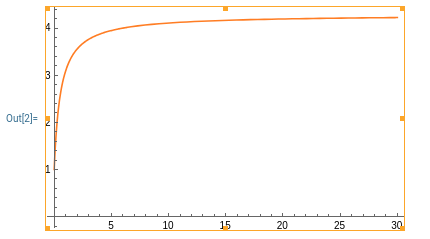
\includegraphics[width=1.0\textwidth]{Alpha of k}
		\caption{Graph of $\alpha(k)$ with $k$ on the $x$-axis. These are parameter values for $(x,\alpha)$ such that equilibria exist in which all vocations are engaged in equilibrium. A complete phase diagram will describe what happens in the economy on either side of the line. That can be done next.}
		\label{fig:my_label}
	\end{figure}
	
	
	
	
	These equilibria are characterized by choosing  
	\begin{align}
		\sigma_0\in\left[\frac{4k+4}{7k+4},\frac{27k+8}{30k+8}\right].\label{Paramter Constraints 2}
	\end{align}
	Notice that if there is no endowment, $k=0$ and everyone enjoys their ``leisure''.
	
	
	
		
\section{Dynamic Extension (Overlapping Generations)}\label{sec:dynamics}

The dynamic stage embeds the static general-equilibrium primitives in a two-period OLG
environment that tracks how \emph{elite-status acquisition} feeds back into production
decisions.  Time is discrete ($t=0,1,2,\dots$).

\subsection{Households}\label{subsec:dyn-households}

A measure-one continuum of identical households is born each period.
An individual born at date~$t$ \emph{lives} for two periods,
consuming the output good $(y_2)$ in each:

\[
U(c_{1t})\;+\;\hat{\beta}\,U(c_{2,t+1}),
\qquad 
U'>0,\;U''<0,\;0<\hat{\beta}<1 .
\]

\paragraph{Budget constraints.}
Let $\alpha\in(0,1]$ denote the fraction of parental wealth transferred to the young
and $k_t$ the dynasty’s stock of the input good $y_1$ at~$t$.
In period~$t$ the young allocate that transfer between current consumption $c_{1t}$
and tuition payments $s_t$ required to purchase a \emph{college membership}
(that is, a unit of the education “good’’ in the static economy).  The effective
price of a tuition unit is $\theta$, a composite of innate ability and inherited social
status; hence

\begin{equation}\label{eq:dyn-B1}
	c_{1t}\;+\;\theta s_t \;=\; \alpha k_t .
\end{equation}

In period $t\!+\!1$ the now-old household finances consumption out of the
return on its earlier tuition investment:

\begin{equation}\label{eq:dyn-B2}
	c_{2,t+1} \;=\; (1+\mathcal{R}_{t+1})\,\theta s_t .
\end{equation}

\paragraph{Optimal tuition demand.}
Maximizing utility \eqref{eq:dyn-B1}–\eqref{eq:dyn-B2} yields the first-order condition

\begin{equation}\label{eq:dyn-FOC}
	U'(\alpha k_t-\theta s_t)
	\;=\;
	\hat{\beta}(1+\mathcal{R}_{t+1})\theta\,
	U'((1+\mathcal{R}_{t+1})\theta s_t),
\end{equation}

which implicitly defines tuition demand

\[
s_t \;=\; \mathcal{F}\!\left(\alpha k_t,\;\theta,\;\mathcal{R}_{t+1}\right).
\]

\subsection{Colleges}\label{subsec:dyn-colleges}

Colleges convert resource inputs into \emph{elite-formation skills}.
An elite college indexed by reputation parameter $\tau\!\in(0,1)$ charges the
tuition fee\footnote{Because $y_1$ is numéraire in the static model we quote all
	tuition and cost figures in units of $y_1$.}
$\tau\alpha k_t$ to screen for highly endowed students.

Per-student cost is increasing and convex, captured by
$(\delta/2)s_t^{\,2}$ with $\delta>0$.  Period-$t$ net income is therefore

\begin{equation}\label{eq:dyn-college-profit}
	\varphi_t \;=\;
	\tau\alpha k_t \;-\;\frac{\delta}{2}s_t^{\,2}.
\end{equation}

Maximizing \eqref{eq:dyn-college-profit} gives the tuition supply schedule

\begin{equation}\label{eq:dyn-college-supply}
	s_t \;=\; \frac{\tau\theta}{\delta},
\end{equation}

and, inverting~\eqref{eq:dyn-college-supply},

\begin{equation}\label{eq:theta-from-s}
	\theta \;=\; \frac{\delta s_t}{\tau}.
\end{equation}

\subsection{Firms}\label{subsec:dyn-firms}

A representative publicly–traded firm chooses capital $k_t$ and
a manager drawn from the education pool.
Stock-holders (all members of the elite) value a particular managerial “style’’
that costs resources $\sigma s_t k_t$ and may conflict with profit maximization.

Let $\aleph(K_t,k_t)$ denote the baseline operating surplus, decreasing in
industry-wide capital $K_t$ and increasing in the firm’s own $k_t$.
With $\varrho_t$ the rental rate of capital (the analogue of $p_2$ in the static section),
profits are

\begin{equation}\label{eq:dyn-firm-profit}
	\pi_t
	\;=\;
	s_t\,\aleph(K_t,k_t)\;-\;\varrho_t k_t\;-\;\sigma s_t k_t .
\end{equation}

First-order optimality yields

\begin{equation}\label{eq:dyn-rental-rate}
	\varrho_t \;=\; s_t\bigl[\aleph_{k_t}(K_t,k_t)\;-\;\sigma\bigr],
\end{equation}

so the return on equity that households anticipate is
$\mathcal{R}_{t+1}=\varrho_{t+1}$.

\subsection{Dynamics and Steady State}\label{subsec:dyn-dynamics}

Combine the household tuition rule \eqref{eq:dyn-FOC},
the supply schedule \eqref{eq:dyn-college-supply},
and the return expression \eqref{eq:dyn-rental-rate}.  Substituting
\eqref{eq:theta-from-s} and $\mathcal{R}_{t+1}$ into \eqref{eq:dyn-FOC} gives the
first-difference equation

\begin{equation}\label{eq:dyn-map}
	s_t \;=\;
	\mathcal{F}\!\!\left(\alpha k_t,\;
	\frac{\delta s_t}{\tau},\;
	s_{t+1}\!\left[\aleph_{k_{t+1}}(K_{t+1},k_{t+1})-\sigma\right]\right),
\end{equation}

which traces an \emph{education locus} in $(s_t,s_{t+1})$-space.
Its slope is

\begin{equation}\label{eq:dyn-slope}
	\frac{\partial s_{t+1}}{\partial s_t}
	\;=\;
	\frac{1-\bigl(\partial\mathcal{F}/\partial\theta\bigr)\,\frac{\delta}{\tau}}
	{ \bigl(\partial\mathcal{F}/\partial \mathcal{R}\bigr)
		\left[\aleph_{k_{t+1}}(K_{t+1},k_{t+1})-\sigma\right] }.
\end{equation}

Intersecting \eqref{eq:dyn-map} with the $45^{\circ}$ line yields the steady-state
tuition level $s^\star$, from which one recovers:
\[
\theta^\star = \frac{\delta s^\star}{\tau},\quad
\mathcal{R}^\star = s^\star\!\left[\aleph_{k}(K^\star,k^\star)-\sigma\right],
\]
and, via \eqref{eq:dyn-B1}–\eqref{eq:dyn-B2}, the corresponding
consumption and wealth profiles.

\medskip
\noindent
\textbf{Interpretation.}  
Because tuition is denominated in the static input good $y_1$, the
dynamic path $(s_t)$ directly feeds back into the general-equilibrium
budget-balance conditions for memberships ($q_1,q_2,\dots$) and hence
into the population shares $(\sigma_0,\sigma_1,\sigma_2)$.  All parameters
($r,\tau,c,\phi,\beta,\alpha$) retain their original static meanings, while
$\hat{\beta},\mathcal{R}_{t+1},\delta$ describe genuinely intertemporal
forces.  (Thus the reader can now move seamlessly from the static to the
dynamic section without a change of notation.)
		
\section{``Referee Report'' \#1 (Claude LLM)}

This paper presents a theoretical analysis of elite status formation and its effects on market equilibrium, addressing the compelling question of why inefficient equilibria persist when elite status commands premium compensation despite potentially lower productivity. The authors develop both a static general equilibrium model using the Ellickson et al.\ (2007) club goods framework and a dynamic overlapping generations extension. While the core economic intuition is strong and the research question highly relevant, the paper requires major revisions to integrate its dual modeling approaches and strengthen its theoretical foundations.

\textbf{Recommendation:} Major revision required.

\subsection{Overall Assessment}

\subsubsection{Research Question and Interest}

The paper tackles a fascinating and important puzzle in economic theory: the persistence of inefficient equilibria in markets where elite institutions and managers command substantial premiums despite questionable productivity advantages. This question resonates strongly with real-world observations about elite universities, consulting firms, investment banks, and other high-status organizations.

The core insight---that status-seeking behavior can create self-sustaining inefficient equilibria---is valuable and merits publication in a top journal. The research question sits at the intersection of several important economic phenomena: signaling, club formation, labor market sorting, and general equilibrium theory.

\subsubsection{Relationship to Existing Literature}

The paper builds appropriately on the Ellickson et al.\ (2007) framework for modeling club goods and group formation. However, the literature review should be strengthened to connect with several other relevant streams:

\begin{itemize}
	\item \textbf{Status signaling models:} The classical work of Spence, Weiss, and others on signaling in labor markets
	\item \textbf{Matching models:} Literature on assortative matching with heterogeneous agents
	\item \textbf{Elite formation:} Sociological and economic work on social mobility and elite reproduction
	\item \textbf{Behavioral economics:} Research on status preferences and social comparison effects
	\item \textbf{Tournament theory:} Models of competition for limited high-status positions
\end{itemize}

A more comprehensive literature review would help position the contribution and identify potential extensions.

\subsection{Technical Assessment}

\subsubsection{The Static General Equilibrium Model}

\paragraph{Strengths}

The static model demonstrates several notable strengths:

\begin{enumerate}
	\item \textbf{Theoretical soundness:} The general equilibrium framework is correctly specified, with proper budget balance conditions for all group types.
	
	\item \textbf{Intuitive structure:} The four-group taxonomy (elite degree mills, serious universities, competent firms, elite firms) effectively captures the essential institutional relationships.
	
	\item \textbf{Clear equilibrium characterization:} The derivation of membership prices and population shares is mathematically sound.
	
	\item \textbf{Valuable numerical example:} The specific parameterization provides useful intuition about equilibrium behavior.
\end{enumerate}

\paragraph{Concerns and Limitations}

Several aspects of the static model warrant attention:

\begin{itemize}
	\item Agent Heterogeneity
	The assumption that all agents are ex-ante identical is quite restrictive. Real-world elite formation typically involves some initial heterogeneity in ability, wealth, or social connections. Introducing such heterogeneity would:
		\begin{itemize}
			\item Make the sorting patterns more realistic
			\item Allow for welfare analysis across different agent types
			\item Potentially generate richer equilibrium dynamics
		\end{itemize}

	\item Utility Function Specification
	The discrete vocational preference structure ($D_1 > D_2 > \ldots > D_5$) feels somewhat ad hoc. The specific values ($D_1 = 32, D_2 = 16, \ldots, D_5 = 2$) appear arbitrary. A more microfounded approach to status preferences would strengthen the analysis, perhaps deriving these rankings from:
		\begin{itemize}
			\item Social interaction effects
			\item Signaling concerns
			\item Network benefits
			\item Consumption complementarities
		\end{itemize}

	\item Institutional Constraints
	The requirement that elite managers must attend elite universities creates the crucial sorting mechanism, but this constraint feels imposed rather than emerging endogenously. It would be more compelling if this constraint arose from:
		\begin{itemize}
			\item Information asymmetries
			\item Network effects
			\item Complementarity in production
			\item Social norms or discrimination
		\end{itemize}
\end{itemize}

\subsection{The Dynamic Extension}

\subsubsection{Major Structural Issues}

The transition from the static to dynamic model presents significant challenges:

\begin{itemize}
	\item Disconnected Frameworks
	Rather than extending the static model, the dynamic section introduces an entirely different modeling approach. The overlapping generations structure, tuition-as-investment mechanism, and firm ownership by elites represent new theoretical elements that don't clearly map back to the static equilibrium conditions.

	\item Inconsistent Notation
The parameter $\theta$ serves different roles across sections, $\beta$ is used for both inefficiency multipliers and discount factors, and the relationship between static membership prices ($q_1, q_2, \ldots$) and dynamic returns ($\mathcal{R}_{t+1}$) remains unclear.

\item Missing Connections
The relationship between static population shares ($\sigma_0, \sigma_1, \sigma_2$) and dynamic tuition decisions ($s_t$) is not established. The steady-state analysis doesn't connect back to the static equilibrium characterization.


\item Specific Technical Problems

\begin{enumerate}
	\item \textbf{Equation \eqref{eq:dyn-map}:} The education locus appears to depend on future values ($s_{t+1}, k_{t+1}$) in a way that may not be consistent with rational expectations.
	
	\item \textbf{Slope analysis in \eqref{eq:dyn-slope}:} The stability conditions are not fully worked out, making it unclear whether the steady state is determinate.
	
	\item \textbf{Welfare implications:} The dynamic model doesn't provide clear insights into efficiency compared to the static analysis.
\end{enumerate}
\end{itemize}

\subsection{Notation and Presentation}

\subsubsection{Cross-Section Consistency}

The notation works reasonably well within each section but becomes problematic when readers need to move between the static and dynamic analyses. Specific issues include:

\begin{itemize}
	\item Parameter overloading ($\beta$, $\theta$)
	\item Unclear variable relationships across models
	\item Missing variable definitions in key equations
\end{itemize}

\subsubsection{Recommendations for Improvement}

\begin{enumerate}
	\item Create a comprehensive notation table that spans both models
	\item Use consistent parameter names throughout
	\item Clarify the mapping between static and dynamic variables
	\item Consider using subscripts or superscripts to distinguish model-specific variables
\end{enumerate}

\subsection{Specific Recommendations}

\subsubsection{Short-term Revisions (Current Draft)}

\begin{enumerate}
	\item \textbf{Model Integration:} Either make the dynamic model a true extension of the static framework, or present them as complementary approaches to the same underlying question with clear connections between their insights.
	
	\item \textbf{Notation Unification:} Ensure that parameters retain consistent meanings throughout the paper. Create a master notation table.
	
	\item \textbf{Welfare Analysis:} Develop a clearer characterization of the efficiency costs of elite equilibria. What is the deadweight loss from status competition?
	
	\item \textbf{Equilibrium Characterization:} Provide more complete conditions for existence and uniqueness of equilibria in both models.
\end{enumerate}

\subsubsection{Medium-term Enhancements (Journal Submission)}

\begin{enumerate}
	\item \textbf{Microfounded Status Preferences:} Replace the ad hoc preference ordering with preferences derived from social interaction, signaling, or network benefits.
	
	\item \textbf{Agent Heterogeneity:} Introduce realistic heterogeneity in initial ability, wealth, or social connections.
	
	\item \textbf{Empirical Relevance:} Add discussion of testable predictions and connections to empirical literature on elite institutions.
	
	\item \textbf{Policy Analysis:} Explore interventions that could improve efficiency: tuition subsidies, regulation of elite institutions, etc.
	
	\item \textbf{Robustness:} Examine how results change under alternative specifications of preferences, technology, or market structure.
\end{enumerate}

\subsection{Addressing the Authors' Specific Questions}

\subsubsection{Does the shift from static to dynamic work?}

In its current form, no. The dynamic model feels like a separate paper rather than an extension of the static analysis. The authors have two viable options:

\begin{itemize}
	\item \textbf{Option A:} Focus exclusively on the static model and develop it more thoroughly, including welfare analysis, comparative statics, and extensions to heterogeneous agents.
	
	\item \textbf{Option B:} Redesign the dynamic model to be a true multi-period version of the static club membership framework, maintaining consistent notation and theoretical foundations.
\end{itemize}

\subsubsection{Should you make the general equilibrium model dynamic?}

This would be extremely challenging but potentially very rewarding. The key would be ensuring that dynamic decisions about education investment are consistent with the static club membership framework. This might involve:

\begin{itemize}
	\item Multi-period memberships with forward-looking agents
	\item Evolution of group compositions over time
	\item Intergenerational transmission of status
	\item Dynamic pricing of memberships
\end{itemize}

Such an approach would likely require a separate paper to develop properly.

\subsubsection{Notation concerns}

Yes, the notation needs significant improvement. The current system works within sections but breaks down across the paper. A unified approach would greatly enhance readability and help readers follow the theoretical development.

\subsection{Minor Comments}

\begin{enumerate}
	\item Page 15: The constraint in equation \eqref{Paramter Constraints 2} should be ``Parameter Constraints''
	\item The figure caption mentions a ``complete phase diagram'' that isn't provided
	\item Some equations could benefit from more detailed derivations in appendices
	\item The transition between sections could be smoother with better introductory paragraphs
\end{enumerate}

\subsection{Conclusion}

This paper addresses an important and fascinating question in economic theory. The core insight about status-driven inefficient equilibria is valuable and novel. The static general equilibrium framework provides a solid foundation for analysis, though it would benefit from extensions to heterogeneous agents and microfounded preferences.

The main weakness is the disconnect between the static and dynamic approaches. Rather than enhancing each other, they currently feel like separate papers. The authors should focus on developing one approach thoroughly rather than attempting to cover both.

Despite these concerns, the underlying research question is compelling enough to warrant publication in a top journal, provided the authors address the integration and theoretical development issues identified above.

The paper would benefit significantly from major revision, but the core contribution is sufficiently valuable to justify the effort required.

\textbf{Final Recommendation:} Conditional acceptance pending major revision.



\section{``Referee Report'' \#2 (GPT 03 LLM)}

The authors have received two referee reports.  
\begin{enumerate}
	\item My \emph{initial report} viewed the paper favourably but highlighted the need for clearer comparative statics, an explicit welfare result, and tighter notation.  I treated the dynamic section as a useful---if schematic---illustration rather than a full‐blown extension.
	\item A \emph{second referee} concurs on most technical points but argues forcefully that the current draft \emph{cannot} sustain two distinct modelling frameworks; they recommend either dropping the OLG or rebuilding the entire paper around it.
\end{enumerate}

Because the authors believe the dynamic perspective is integral, this consolidated report reassesses the manuscript \emph{under the assumption that both the static GE and the dynamic OLG must remain}.  I identify what must happen for a dual‐model approach to survive peer review at a top economics journal.

\bigskip
\hrule
\bigskip

\subsection{High–Level Evaluation}

\begin{description}
	\item[Research question.] \emph{Why do resource‐wasting elite institutions persist in competitive markets?}  
	This is timely, policy‐relevant, and under‐explored in the formal GE literature.
	
	\item[Core contribution.]  A club‐good GE à la \citet{Ellickson1999} that endogenises tuition, labour sorting, and membership prices, \emph{plus} an OLG overlay that turns tuition into an intergenerational investment and feeds back into firm behaviour through a “style’’ cost.
	
	\item[Novelty.]  The static model alone is a fresh application of club equilibrium to elite status.  
	The OLG adds insight into \emph{wealth dynamics} and into how status‐based rents are recycled across generations—an angle largely absent from the recent positional‐goods literature.  
	
	\item[Feasibility of a two‐model paper.]  Viable \emph{provided} the authors:
	\begin{enumerate}%[(i)]
		\item establish a transparent mapping from static objects $(p,q,\sigma)$ to dynamic variables $(s,\mathcal R,k)$;
		\item show the static equilibrium is the \emph{per‐period allocation} arising in the dynamic steady state;
		\item prove at least one proposition in which the comparative statics of the static model coincide with the slope of the OLG locus (\emph{consistency property}).
	\end{enumerate}
\end{description}

\bigskip
\hrule
\bigskip

\subsection{Detailed Strengths and Weaknesses}

\subsubsection{Static General‐Equilibrium Block}

\paragraph{Strengths.}
\begin{itemize}
	\item Elegant encoding of education and employment as priced memberships.
	\item Closed‐form interior solution (membership prices, population shares) yields intuitive comparative statics in $k$, $\alpha$, $\beta$, and $\tau$.
	\item Numerical example gives the reader concrete intuition.
\end{itemize}

\paragraph{Key deficiencies to fix.}
\begin{enumerate}%[(S1)]
	\item \emph{Existence/uniqueness}: Provide a theorem citing Ellickson’s conditions and show that your special utility (piecewise‐linear in status) satisfies them.  
	\item \emph{Welfare}: Insert a proposition that the equilibrium is Pareto‐inefficient whenever $\alpha\beta<1$ or $\tau>1$ (deadweight loss from burnt resources).
	\item \emph{Heterogeneity}: At minimum introduce a one‐dimensional type (ability or wealth) to show that sorting continues to hold.  A simple two‐type appendix suffices.
	\item \emph{Microfounded preference ordering}: Replace ad‐hoc $D_i$’s with a separable utility $U(y_1,y_2)+\eta\,\text{Status}$ where $\eta$ is a parameter.  Normalise $\eta$ to reproduce the ranking $D_1>\dots>D_5$.
\end{enumerate}

\subsubsection{Dynamic OLG Block}

\paragraph{Strengths.}
\begin{itemize}
	\item Converts tuition into an intertemporal choice and links it to firm returns.
	\item Offers a channel through which rising macro wealth $k_t$ can expand the share of elites---an empirically plausible mechanism.
\end{itemize}

\paragraph{Critical gaps (must be closed).}
\begin{enumerate}%[(D1)]
	\item \emph{Mapping to static equilibrium}: Show formally that if $s_t=s^\star$, then the induced membership prices $q^\star$ and shares $\sigma^\star$ satisfy the static equilibrium conditions.  (One lemma plus an algebraic mapping table.)
	\item \emph{Notational collisions}: Reserve Greek letters for \emph{parameters} and Latin for \emph{endogenous variables}.  Concretely:
	\[
	\beta\ (\text{static inefficiency}) \;\longrightarrow\; \xi,\qquad
	\hat{\beta}\ (\text{discount}) \;\longrightarrow\; \beta.
	\]
	Similar fixes for $\alpha,\theta,\sigma$.
	\item \emph{Stability of steady state}: Provide the Jacobian of the two‐dimensional system in $(k_t,s_t)$ and state a proposition: “If $\partial s_{t+1}/\partial s_t<1$ and $\partial k_{t+1}/\partial k_t<1$, the steady state is locally stable.’’
	\item \emph{Link to welfare}: Define a dynastic utilitarian criterion and show the steady state is (generically) not first‐best due to status externalities.
\end{enumerate}

\bigskip
\hrule
\bigskip

\subsection{Integration Blueprint for a Unified Paper}

Below is a concrete road‐map the authors can follow to convince sceptical referees that the two blocks belong in the \emph{same} manuscript.

\begin{enumerate}%[A.]
	\item \textbf{Master Notation Table (1 page).}  
	Two panels: \emph{Parameters} $(k_0,r,\tau,\xi,\alpha,\dots)$ and \emph{Endogenous variables} $(p,q,\sigma,s,k_t,\mathcal R_t)$ with a column indicating “Static”, “Dynamic”, or “Both”.
	
	\item \textbf{Section~2: Static GE}  
	\begin{itemize}
		\item Assumptions, existence theorem, welfare proposition.
		\item Comparative statics Cor.\ 1: $\partial\sigma_1/\partial k$, $\partial\sigma_1/\partial\xi$, etc.
	\end{itemize}
	
	\item \textbf{Section~3: Dynamic OLG}  
	\begin{itemize}
		\item Show how tuition $s_t$ generates membership prices via $q_1=q(s_t),\dots$.
		\item Lemma~1 (Consistency): If $s_t=s^\star$, then $(p,q,\sigma)$ coincide with static equilibrium.
		\item Proposition~2: Steady‐state existence and local stability.
		\item Cor.\ 2: The sign of $\partial s^\star/\partial k_0$ matches sign of $\partial\sigma_1/\partial k$ (harmonising comparative statics).
	\end{itemize}
	
	\item \textbf{Section~4: Discussion and Policy}.  
	Highlight novel insights obtainable \emph{only} with the dynamic overlay: e.g.\ wealth‐induced “elite explosion,” path dependence, and possible policy levers (tuition taxes).
\end{enumerate}

\bigskip
\hrule
\bigskip

\subsection{Concrete Action Items Before Resubmission}

\begin{enumerate}%[(i)]
	\item \textbf{Unify notation} per Section~4.A.
	\item \textbf{Add two formal propositions} (welfare inefficiency in static; stability in dynamic).
	\item \textbf{Provide a short literature subsection} linking to signalling, matching, positional externalities, and human‐capital OLG.
	\item \textbf{Revise numerical example} so that parameters satisfy new heterogeneity and stability conditions; plot both the static shares and the OLG phase diagram.
	\item \textbf{Supply an online appendix} with algebra for membership prices, Jacobian calculations, and robustness checks (\emph{η‐variant preferences}, alternative production functions).
\end{enumerate}

\bigskip
\hrule
\bigskip

\subsection{Final Recommendation}

Retain \emph{both} modelling blocks, but weld them together following the blueprint above.  
Successful execution would yield a distinctive contribution: a microfounded explanation for the intergenerational persistence of inefficient status institutions within a competitive GE, backed by rigorous comparative statics and welfare analysis.

\bigskip
\textbf{Verdict:} \emph{Invite a major revision that integrates the static GE and dynamic OLG as outlined.}

	
	\bibliographystyle{plainnat}
	\bibliography{references} 
	
\end{document}
